\chapter{Исследование наблюдаемости}
\label{ch:chap3}
\section{Условие задачи}

Рассматриваем систему:
$$
  \begin{cases}
    \dot{x} = Ax \\
    y = Cx
  \end{cases}
$$ и выполнить следующие шаги:


    Исследовать наблюдаемость системы:
      \begin{itemize}
        \item Найти матрицу наблюдаемости системы, определить ее ранг, сделать вывод об наблюдаемости системы в целом.
        \item Найти собственные числа матрицы A, найти для каждого из собственных чисел матрицу Хаутуса 
        (для наблюдаемости), определить ранги матриц, сделать
         выводы об наблюдаемости каждого собственного числа и системы в целом.
         \item Найти Жорданову (или диагональную) форму системы и сделать выводы об
         наблюдаемости каждого собственного числа и системы в целом.
      \end{itemize}
      
      Найти Грамиан наблюдаемости системы относительно времени $t_1 = 3$, вычислить
      его собственные числа. Проанализировать полученные собственные числа с точки
      зрения наблюдаемости системы.

      Считая, что выход системы $y(t)$ подчиняется закону $y(t) = f(t)$ на временном
      интервале $t\in[0,t_1]$ определить начальные условия системы. Выполнить моделирование системы, 
      демонстрирующее корректность выполненных расчетов.
    

\section{Решение задачи}

Параметры для объекта:
$$
  A = \begin{bmatrix}
    8   &	-3	&  -12 \\
    -3   &   -2  &  -6 \\
    6  &    0  &  7
  \end{bmatrix} \tab
  C = \begin{bmatrix}
    1\\0\\2 
  \end{bmatrix}^T \tab
  f(t) = 2e^{-2t}cos(3t) + e^{-2t}sin(3t)
$$



\subsection{Исследование наблюдаемости системы}
Для начала найдём матрицу наблюдаемости системы:
$$
V = \begin{bmatrix}
    C \\ CA \\ CA^2
\end{bmatrix} = \begin{bmatrix}
                1   &	0	&  2 \\
                4   &   -3  &  2 \\
                -11  &    -6  &  16
            \end{bmatrix}
$$
$$
  rank(V) = 3
$$
По критерию Калмана, наша система полностью наблюдаема , так как ранк матрицы наблюдаемости равен порядку системы.

Найдём собственные числа матрицы $A$:
$$
    \lambda_{1,2} = -2 \pm 3i, \tab \lambda_3 = 1 
$$

Вычислим матрицу Хаутуса для каждого собственного числа:
$$
    H_1 = \begin{bmatrix}
          A - \lambda_1 I \\ C   
          \end{bmatrix} = 
    \begin{bmatrix}
    -6-3i & -3 & -12  \\  
      -3 & -3i & -6  \\  
     6 & 0 & 9-3i \\ 
      1 & 0 & 2
    \end{bmatrix}
$$
$$
rank(H_1) = 3
$$
Значит собственное число $\lambda_1$ является наблюдаемым, если ранг его матрицы Хаутуса равняется порядку системы.
$$
    H_2 = \begin{bmatrix}
          A - \lambda_2 I \\ C
          \end{bmatrix} = 
        \begin{bmatrix}
            -6+3i & -3 & -12  \\  
              -3 & +3i & -6  \\  
             6 & 0 & 9+3i \\ 
              1 & 0 & 2
        \end{bmatrix}
$$
$$
rank(H_2) = 3
$$
Аналогично, собственное число $\lambda_2$ является наблюдаемым.
$$
    H_3 = \begin{bmatrix}
          A - \lambda_3 I \\ C   
          \end{bmatrix} = 
        \begin{bmatrix}
            -9 & -3 & -12  \\  
              -3 & -3 & -6  \\  
             6 & 0 & 6 \\ 
              1 & 0 & 2
        \end{bmatrix}
$$
$$
rank(H_3) = 3
$$
Аналогично, собственное число $\lambda_3$ является наблюдаемым. Как следствие - система полностью наблюдаема.

Теперь найдём Жорданову форму системы, в общем виде она выглядит следующим образом:
$$
    \begin{cases}
      \dot{\hat{x}} = P^{-1}\boldsymbol{A}P \hat{x} + P^{-1}\boldsymbol{B} u \\
      y = CP\hat{x}
    \end{cases}
$$

Система в жордановой форме полностью наблюдаема тогда и только тогда, когда
\begin{itemize}
  \item Все жордановы клетки относятся к различным собственным числам
  \item Элементы матрицы выходов, соответствующие первым столбцам жордановых клеток, не равны нулю.
\end{itemize}

В нашем случае жорданова клетка и выходное воздействие таково:
$$
    \mathbf{A} = \begin{bmatrix}
        1 & 0 & 0 \\
        0 & -2 & -3 \\
        0 & 3 & -2 
        \end{bmatrix} \tab 
$$
$$
CP = C^* = \begin{bmatrix}
    1 & 0.5-0.5i & 0.5+0.5i 
    \end{bmatrix}
$$

Как можно заметить, оба собственных числа соответствуют различным жордановым клеткам, и для каждой из них
первый столбец матрицы выходных воздействий не равен нулю, поэтому все собственные числа наблюдаемые и система полностью наблюдаема.

\subsection{Грамиан наблюдаемости}

Грамиан наблюдаемости системы относительно времени $t_1 = 3$:

$$
Q(t_1) = \int_{0}^{t_1}e^{A^Tt}C^TCe^{At}dt = 
    \begin{bmatrix}
        201.92 & -201.35 & 202.09 \\
        -201.35 & 201.15 & -201.30 \\
        202.09 & -201.30 & 202.42
    \end{bmatrix}
$$

Его собственные числа:
$$
    q_{1} = 605.006 , \tab q_{2} = 0.007, \tab q_3 = 0.492
$$
Получается, все собственные числа положительны, а это значит, что матрица Грамиана является положительно определённой, 
значит система  полностью наблюдаема.

\newpage
\subsection{Определение начальных условий}

Будем считать, что выход системы соответствует заранее заданной функции: $f(t) = y(t) = 2e^{-2t}cos(3t) + e^{-2t}sin(3t)$

Посчитаем вектор начальных условий:
$$
    x(0) = (Q(t1))^{-1}\int_{0}^{t_1}e^{A^Tt}C^Ty(t)dt = 
    \begin{bmatrix}
        0\\1\\1
    \end{bmatrix}
$$

Вектор состояний системы будет выглядеть следующим образом:
\begin{figure}[ht]
  \centering
  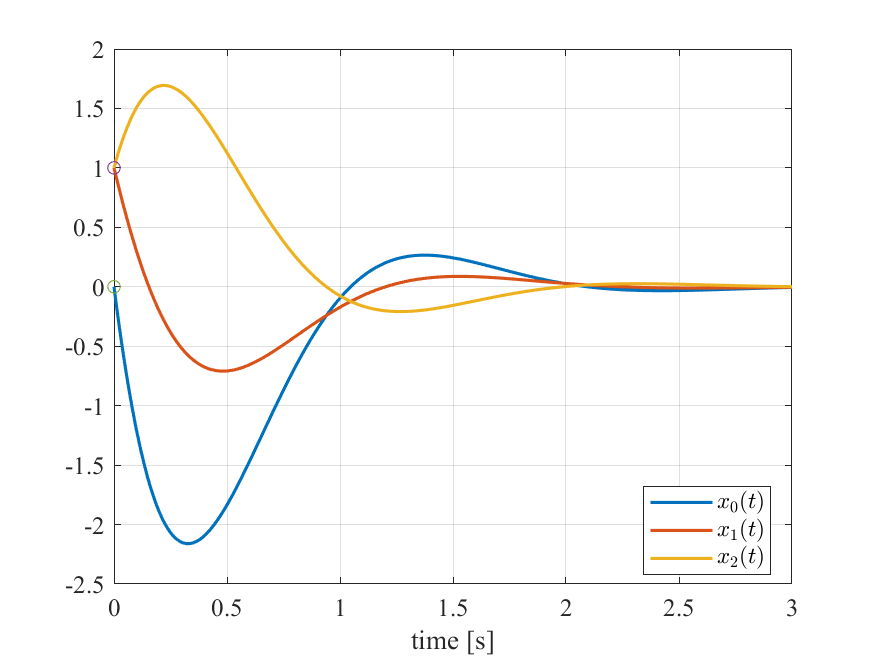
\includegraphics[width=1.0\textwidth]{observability1.png}
  \caption{Состояния системы}
\end{figure}

Как можно заметить, они совпадают с моделированием вектора состояний.
\newpage
Теперь проведём моделирование с начальными условиями x(0), без управления: на рисунке ниже видно,
что выход системы совпадает с функцией y(t) выше заданной. Ошибка наблюдения достаточно мала и не превышает $10^{-10}$.

\begin{figure}[ht]
    \centering
    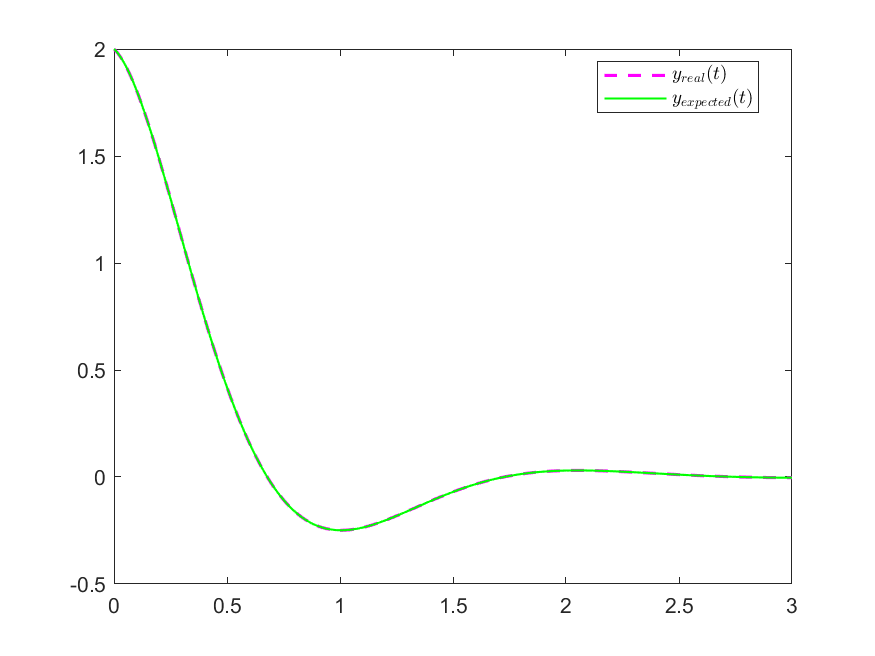
\includegraphics[width=1.0\textwidth]{output1.png}
    \caption{Выход системы}
  \end{figure}

\begin{figure}[ht]
    \centering
    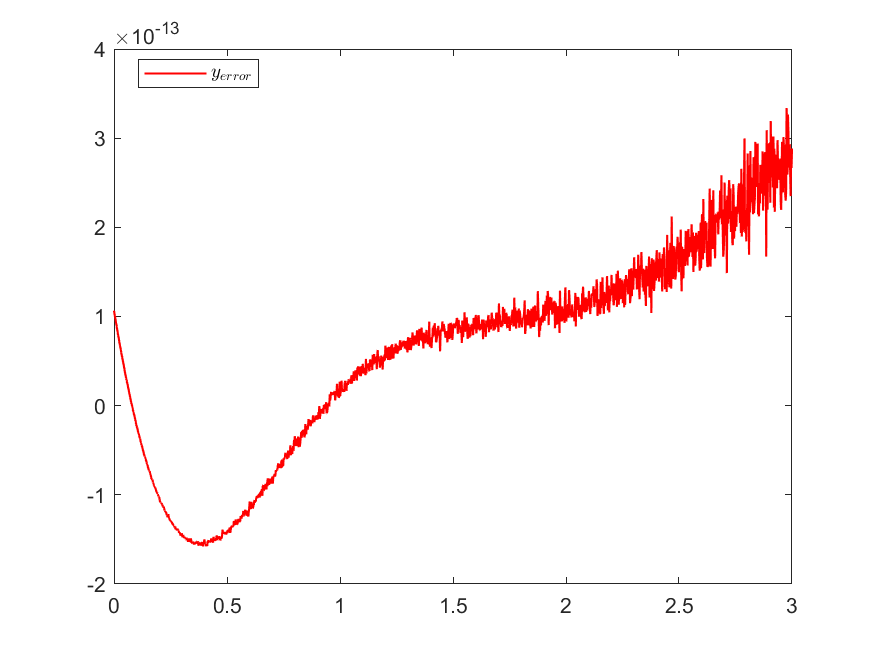
\includegraphics[width=1.0\textwidth]{error1.png}
    \caption{Ошибка выхода системы}
  \end{figure}

\newpage
\subsection{Вывод}
В этом задании нам удалось показать, что система является полностью наблюдаемой. 
Это было показано с помощью матрицы  наблюдаемости, через наблюдаемость собственных значений и жорданову форму системы.
Также был найден грамиан наблюдаемости и проверены его собственные числа. 
Провели моделирование системы с начальными условиями, при которых выход системы совпадает
с заданной функцией. Результаты моделирования показали, что система наблюдаема и
наблюдение работает корректно.

\endinput